\section{Objectives}
\label{sec:Objectives}

In this thesis, we propose a new tool-supported workflow in which client code gets automatically migrated after a web service was modified. We focus on light-weight Web API technologies which can be described by an IDL, such as REST, GraphQL and gRPC. Our main objective is to facilitate the workflow shown in Figure \ref{fig:oldWorkflow} by significantly reducing the effort for API consumers. Therefore, we introduce a state-of-the-art description language to specify a machine-readable migration guide. This guide enables API providers to describe all modifications of a Web API from a previous to its latest version. In addition, we propose a tool that parses our migration guide and generates library code that is persistent to changes to its public interface once it is run for the first time. It can be used in an existing \ac{CI/CD} pipeline or via the command line.

\begin{figure}[h]
	\centering{
		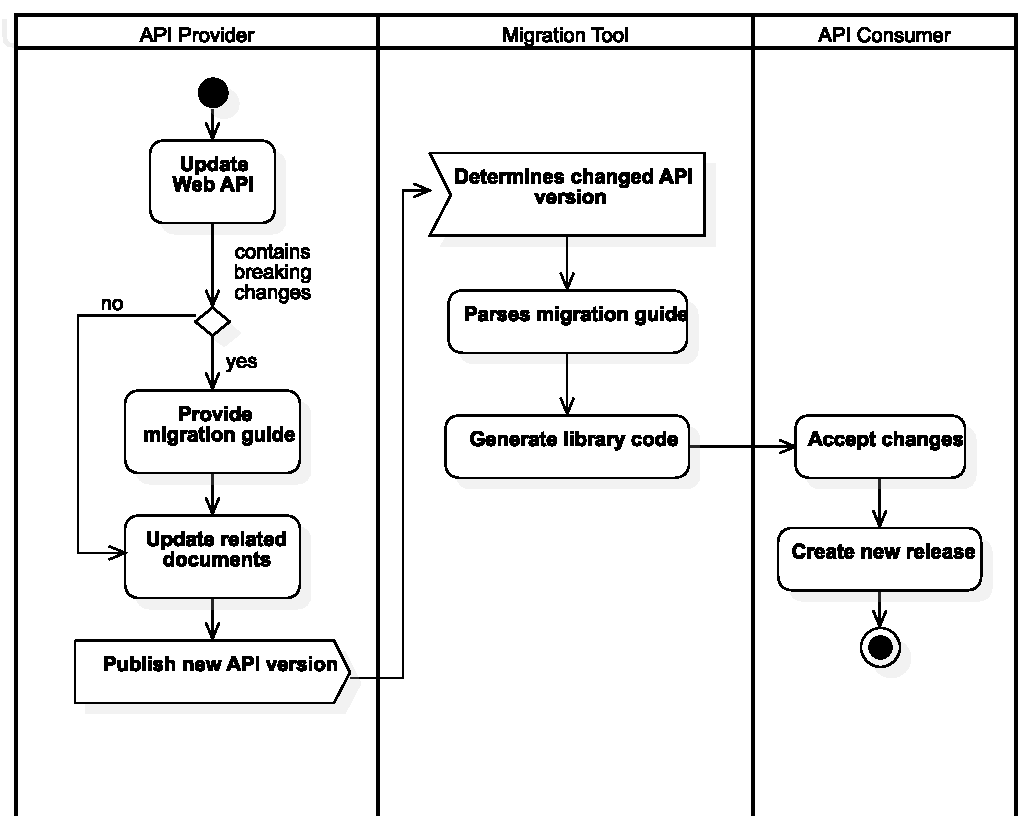
\includegraphics[width=128mm]{images/new_workflow.pdf}
		\caption{Workflow with tool support after web service changes}
		\label{fig:newWorkflow}
	}
\end{figure}

Figure \ref{fig:newWorkflow} showcases the new workflow. In addition to their current tasks, Web API providers must state all introduced changes in a machine-readable migration guide and make it available to consumers. Web API consumers have to integrate our migration tool, which automates the incorporation of changes without breaking the client application. It determines the API version from the migration guide and creates a set of rules indicating how the library should be customized to avoid introducing breaking changes to the consumer's application code. After executing these rules, the public interface of the generated library code remains unchanged and the consumer's application continues to use the library's code which acts as a facade for the lower level API calls.